\Chapter{Tesztelés}

A tesztelési fejezet részletesen bemutatja az Acxor rendszer tesztelési stratégiáját, az alkalmazott eszközöket, a tesztesetek felépítését és az elért eredményeket. A tesztelés célja annak igazolása, hogy az implementált funkciók az elvárásoknak megfelelően működnek, és hogy a jövőbeli módosítások regressziót ne okozzanak a meglévő működésben.

% ─────────────────────────────────────────────────────────────────────────────
\Section{Tesztelési stratégia}
% ─────────────────────────────────────────────────────────────────────────────

A rendszer tesztelése két jól elkülönített rétegben valósult meg. A backend oldalon integrációs tesztek ellenőrzik a teljes kérés-válasz ciklust, beleértve az adatbázissal való interakciót, a hitelesítési logikát és az üzleti szabályok érvényesítését. A frontend oldalon egységtesztek verifikálják az állapotkezelési logikát, az action creator függvényeket és a legfontosabb UI komponensek helyes renderelését.

A tesztelési megközelítés a következő elveket követi:
\begin{itemize}
  \item Minden teszteset független és izolált: a tesztek között nincs közös állapot, az adatbázis tartalma minden teszteset után törlődik.
  \item A tesztek lehetőség szerint a rendszer külső viselkedését ellenőrzik, nem belső implementációs részleteket.
  \item A tesztek a fejlesztéssel párhuzamosan készültek, nem utólag.
  \item Ahol a külső rendszerek (GitHub API) nem hívhatók valódi tesztekben, mockolt adatokkal dolgozunk.
\end{itemize}

% ─────────────────────────────────────────────────────────────────────────────
\Section{Backend tesztelés}
% ─────────────────────────────────────────────────────────────────────────────

\SubSection{Eszközök és konfiguráció}

A backend tesztek Jest tesztelési keretrendszert és Supertest HTTP tesztkönyvtárat alkalmaznak. A Jest biztosítja a tesztfuttatót, az assertionokat és a mock funkcionalitást. A Supertest lehetővé teszi, hogy az Express alkalmazásnak valódi HTTP kéréseket küldjünk anélkül, hogy portot kellene foglalni, így a tesztek gyorsan és izoláltan futnak.

Az adatbázis szintű izoláció érdekében a \texttt{mongodb-memory-server} könyvtár egy in-memory MongoDB példányt indít el minden tesztfájl futtatásakor. Ez azt jelenti, hogy a tesztek semmilyen körülmények között nem érintik az éles vagy fejlesztési adatbázist. A \texttt{\_\_tests\_\_/setup.ts} fájl konfigurálja ezt a mechanizmust, és a Jest \texttt{globalSetup} vagy \texttt{setupFilesAfterEnv} konfigurációján keresztül kerül betöltésre.

\SubSection{Auth tesztek}

A hitelesítési tesztek a \texttt{POST /api/auth/register} és \texttt{POST /api/auth/login} végpontokat fedik le. A regisztrációs tesztek ellenőrzik:

\begin{itemize}
  \item Sikeres regisztráció esetén 201-es státuszkód és érvényes JWT token visszaadása.
  \item A jelszó nem jelenik meg a válaszban (adatbiztonság).
  \item Duplikált e-mail esetén 400-as hiba és megfelelő üzenet visszaadása.
  \item A visszaadott token érvényes JWT formátumú (három pontosvesszővel elválasztott Base64 szegmens).
  \item Az alapértelmezett XP és level értékek helyesek (\texttt{xp: 0}, \texttt{level: 1}).
\end{itemize}

A bejelentkezési tesztek ellenőrzik a helyes adatokkal való sikeres bejelentkezést, a helytelen jelszóra adott 400-as választ, a nem létező e-mailre adott hibaüzenetet, és azt, hogy bejelentkezés válaszában sem szerepel a jelszó.

\begin{lstlisting}[language=JavaScript, caption={Regisztrációs teszt részlet (auth.test.ts)}]
it('a jelszó nem kerül vissza a válaszban', async () => {
  const res = await request(app)
    .post('/api/auth/register')
    .send(validUser);

  expect(res.body.user).not.toHaveProperty('password');
});

it('a visszaadott token érvényes JWT formátumú', async () => {
  const res = await request(app)
    .post('/api/auth/register')
    .send(validUser);

  const jwtPattern =
    /^[A-Za-z0-9-_]+\.[A-Za-z0-9-_]+\.[A-Za-z0-9-_]+$/;
  expect(res.body.token).toMatch(jwtPattern);
});
\end{lstlisting}

\SubSection{Projekt tesztek}

A projekt tesztek a teljes CRUD ciklust lefedik. Minden teszteset saját felhasználót regisztrál (\texttt{registerAndLogin} segédfüggvény), így biztosítva az izolációt. A lefedett esetek:

\begin{itemize}
  \item Projekt létrehozása helyes adatokkal (201), token nélkül (401), hiányzó névvel (400).
  \item A létrehozó automatikusan adminisztrátor és tag lesz.
  \item TaskGroup-okkal való projektlétrehozáskor a feladatok és alfeladatok létrejönnek az adatbázisban.
  \item Érvénytelen tokennel való kísérlet 401-et ad vissza.
  \item A projektek listázása csak a saját projektek tartalmazza (más felhasználóé nem jelenik meg).
  \item Az admin mező populálva érkezik vissza (jelszó nélkül).
  \item Projekt módosítása és törlése csak az adminisztrátornak engedélyezett (másnak 403).
  \item Törléskor a kapcsolódó feladatok és alfeladatok is törlődnek.
\end{itemize}

\begin{lstlisting}[language=JavaScript, caption={Projekt törlési teszt (projects.test.ts)}]
it('törli a projektet és az összes kapcsolódó task-ot', async () => {
  const createRes = await request(app)
    .post('/api/projects')
    .set('Authorization', `Bearer ${token}`)
    .send({
      name: 'Törlendő projekt',
      taskGroups: [{
        name: 'Sprint 1', deadline: '2025-07-01',
        tasks: [{ description: 'Törlendő task',
                   subtasks: ['Sub 1'] }],
      }],
    });

  const projectId = createRes.body._id;

  const deleteRes = await request(app)
    .delete(`/api/projects/${projectId}`)
    .set('Authorization', `Bearer ${token}`);

  expect(deleteRes.status).toBe(200);

  const remainingTasks = await Task.find({ project: projectId });
  expect(remainingTasks).toHaveLength(0);
});
\end{lstlisting}

\SubSection{Feladat tesztek}

A task tesztek a feladatok létrehozását, lekérését, módosítását és törlését fedik le. Fontos tesztesetek:

\begin{itemize}
  \item A feladat alapértelmezett státusza \texttt{'Open'}.
  \item A határidő (\texttt{deadline}) helyesen tárolódik és visszaadódik.
  \item A státusz módosítható (pl. \texttt{'Open'} $\rightarrow$ \texttt{'InProgress'}).
  \item Törlés után a feladat nem jelenik meg a projekt feladatlistájában.
  \item Token nélküli hozzáférés 401-es hibát ad.
\end{itemize}

\SubSection{Alfeladat tesztek}

Az alfeladat tesztek hasonló struktúrát követnek, mint a feladattesztek, kiegészítve az XP alapértékének ellenőrzésével (\texttt{xpReward: 0}) és az XP mező módosíthatóságával.

\SubSection{Service tesztek}

\textbf{xpService tesztek}: Az \texttt{addXP} függvény tesztelése az in-memory adatbázison fut (nem mockolt), így valódi Mongoose dokumentumokon ellenőrizzük a viselkedést. A tesztesetek:

\begin{itemize}
  \item XP hozzáadásakor az érték helyesen növekszik.
  \item Küszöbérték elérésénél szintlépés következik be (maradék XP-vel).
  \item Több szintlépés egyszerre is működik.
  \item Nulla XP hozzáadása nem változtatja meg az állapotot.
  \item Nem létező felhasználóra hiba dobódik (\texttt{'User not found'}).
  \item A szint és XP az adatbázisban is perzisztálódik.
  \item Pontosan a küszöbön lévő XP szintlépést okoz, maradék 0 XP-vel.
\end{itemize}

\begin{lstlisting}[language=JavaScript, caption={XP szintlépési teszt (xpService.test.ts)}]
it('több szintet lép egyszerre, ha sok XP érkezik', async () => {
  const user = await createUser(0, 1);
  // 1. szint: 100 XP, 2. szint: 200 XP -> 300 XP kell a 3. szinthez
  const updated = await addXP(user._id.toString(), 350);

  expect(updated.level).toBe(3);
  expect(updated.xp).toBe(50);
});
\end{lstlisting}

\textbf{githubService tesztek}: Az axios modul teljes mocking-jával teszteljük, hogy a service a helyes GitHub API URL-eket hívja-e, a helyes Authorization headert küldi-e el, és a válasz adatait a várt formátumra alakítja-e (pl. \texttt{creator} mező a \texttt{user.login}-ból).

\textbf{logService tesztek}: A \texttt{console.log} spy-olásával ellenőrizzük, hogy a naplóbejegyzések a várt formátumban (\texttt{[PROJECT id] üzenet}) kerülnek kiírásra. Ez a teszt a log mentési logikát is verifikálja, de mivel a log service az adatbázisba is ír, a tesztek in-memory DB-n futnak.

% ─────────────────────────────────────────────────────────────────────────────
\Section{Frontend tesztelés}
% ─────────────────────────────────────────────────────────────────────────────

\SubSection{Eszközök és konfiguráció}

A frontend tesztek Vitest tesztelési keretrendszert és React Testing Library-t alkalmaznak. A Vitest Vite-alapú, és natívan kezeli a TypeScript-et és a JSX-et. A React Testing Library a komponensek felhasználói szemszögből való tesztelésére ösztönöz: nem az implementáció részleteit, hanem a látható és interakcióra képes elemeket ellenőrzi.

A tesztek konfigurációja a Vitest konfigurációs fájlban a \texttt{jsdom} tesztkörnyezetet alkalmazza, a \texttt{@testing-library/jest-dom} pedig bővíti a matchers listát (pl. \texttt{toBeInTheDocument}, \texttt{toHaveProperty}).

\SubSection{Reducer tesztek}

A reducer tesztek a legegyszerűbbek: tiszta függvényeket tesztelnek, amelyeknek nincs mellékhatásuk. Az \texttt{AppReducer} tesztjei ellenőrzik a \texttt{SET\_SUBTASKS}, \texttt{SET\_LOADING} és \texttt{SET\_SELECTED\_PROJECT} action típusokat. A \texttt{ViewReducer} tesztjei verifikálják az ismeretlen action típusra adott alapértelmezett viselkedést, és az összes \texttt{ViewState} értékkel való kompatibilitást.

\begin{lstlisting}[language=JavaScript, caption={ViewReducer tesztek (ViewReducer.test.tsx)}]
it('SET_VIEW akció frissíti az activeView-t', () => {
  const action: ViewAction = { type: 'SET_VIEW', payload: 'tasks' };
  const newState = ViewReducer(initialViewState, action);
  expect(newState).toBe('tasks');
});

it('többféle ViewState-et is kezel', () => {
  const states: ViewState[] =
    ['main', 'kanban', 'scrum', 'subtasks', 'log'];
  states.forEach((state) => {
    const newState = ViewReducer(initialViewState,
      { type: 'SET_VIEW', payload: state });
    expect(newState).toBe(state);
  });
});
\end{lstlisting}

\SubSection{Context tesztek}

A Context tesztek egyszerű tesztkomponenseket renderelnek a Context Providerbe ágyazva, és ellenőrzik az alapértelmezett állapotot, majd egy gombnyomás szimulációjával a dispatch utáni állapotváltozást.

\begin{lstlisting}[language=JavaScript, caption={GlobalContext integrációs teszt}]
it('dispatch frissíti a token-t és user-t', () => {
  render(
    <GlobalProvider>
      <TestComponent />
    </GlobalProvider>,
  );

  fireEvent.click(screen.getByText('Set User'));
  expect(screen.getByText('Token: abc123')).toBeInTheDocument();
});
\end{lstlisting}

\SubSection{Action tesztek}

Az action tesztek az axios mock-olásával ellenőrzik, hogy a \texttt{fetchTasks} és \texttt{addTask} függvények a helyes URL-t hívják-e, a megfelelő headereket küldik-e el, és a szerver válasza alapján a helyes dispatch hívásokat indítják-e el. Hibaeset szimulációjával ellenőrizzük a \texttt{SET\_ERROR} dispatch-t is.

\SubSection{Komponens tesztek}

\textbf{Sign komponens}: A tesztek ellenőrzik, hogy mindkét form (Register és Login) renderelésre kerül, a form submit az adatokkal meghívja a megfelelő action függvényt, és a loading / error állapotok megjelennek a felületen.

\textbf{CreateProject komponens}: A tesztek verifikálják a kezdő lépés megjelenítését, a Manual flow következő lépésre váltást, a contributor hozzáadás működését, és hogy üres contributor nem adható hozzá.

\textbf{TasksView és SubTasksView komponensek}: Mockolt globális állapottal ellenőrzik, hogy a feladatok és alfeladatok cím szerint megjelennek-e a nézetben.

\textbf{Sidebar és Topbar}: Strukturális tesztek ellenőrzik, hogy a megfelelő számú gomb és a várt HTML elem (\texttt{header} szerepkör) megjelenik-e.

\begin{table}[h!]
\centering
\small
\begin{tabularx}{\textwidth}{|l|Y|c|}
\hline
\textbf{Tesztkészlet} & \textbf{Lefedett esetek} & \textbf{Tesztek száma} \\
\hline
auth.test.ts & Regisztráció, bejelentkezés, token validáció & 9 \\
projects.test.ts & CRUD, jogosultság, taskGroup import & 11 \\
tasks.test.ts & CRUD, állapotváltás, határidő kezelés & 8 \\
subtasks.test.ts & CRUD, alapértékek, XP mező & 8 \\
xpService.test.ts & XP hozzáadás, szintlépés, perzisztencia & 8 \\
githubService.test.ts & API hívások, adat transzformáció & 11 \\
logService.test.ts & Naplóformátum, userId kezelés & 5 \\
app.test.ts & Alapvető route ellenőrzés & 1 \\
\hline
\textbf{Backend összesen} & & \textbf{61} \\
\hline
Reducer.test.tsx & AppReducer action típusok & 3 \\
ViewReducer.test.tsx & ViewReducer állapotváltás & 3 \\
GlobalContext.test.tsx & Context alapállapot, dispatch & 2 \\
ViewContext.test.tsx & View váltás dispatch-csel & 2 \\
Actions.test.ts & fetchTasks, addTask, hibakezelés & 3 \\
Sign.test.tsx & Form render, submit, loading/error & 4 \\
CreateProject.test.tsx & Lépések, contributor kezelés & 4 \\
TasksView.test.tsx & Feladatlista renderelés & 1 \\
SubTasksView.test.tsx & Alfeladatlista renderelés & 1 \\
Sidebar.test.tsx & Ikonok száma & 1 \\
Topbar.test.tsx & Banner elem & 1 \\
\hline
\textbf{Frontend összesen} & & \textbf{25} \\
\hline
\textbf{Összes teszteset} & & \textbf{86} \\
\hline
\end{tabularx}
\caption{A tesztkészletek összefoglalása}
\label{tab:test-summary}
\end{table}

% ─────────────────────────────────────────────────────────────────────────────
\Section{Manuális tesztelés}
% ─────────────────────────────────────────────────────────────────────────────

Az automatizált tesztek mellett a rendszer manuális tesztelésen is átesett. Ennek során a következő folyamatokat ellenőriztük végig a böngészőben és fizikai mobil eszközön:

\begin{itemize}
  \item Teljes regisztráció és bejelentkezés folyamata.
  \item Projekt létrehozása manuálisan és GitHub importtal.
  \item Feladatok és alfeladatok hozzáadása, szerkesztése, törlése és befejezése.
  \item XP jóváírás és szintlépés ellenőrzése a főoldalon és a gamification nézetben.
  \item Sprint létrehozása, feladat hozzárendelése és sprint törlése.
  \item Belső levelezés küldése és fogadása két különböző felhasználói fiókkal.
  \item Aktivitásnapló megjelenítésének ellenőrzése különböző műveletek elvégzése után.
  \item Profil szerkesztés (felhasználónév, e-mail, jelszó módosítás).
  \item Mobil alkalmazás teljes funkcionalitásának ellenőrzése Android eszközön (Expo Go).
\end{itemize}

\begin{figure}[h!]
\centering
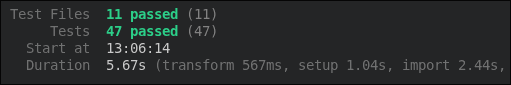
\includegraphics[width=0.8\textwidth]{images/vitest_results.png}
\caption{A frontend unit tesztek futtatásának eredménye (Vitest)}
\label{fig:architecture}
\end{figure}

\begin{figure}[h!]
\centering
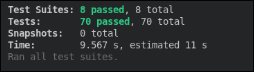
\includegraphics[width=0.8\textwidth]{images/jest_results.png}
\caption{A backend integrációs tesztek futtatásának eredménye (Jest)}
\label{fig:architecture}
\end{figure}

% ─────────────────────────────────────────────────────────────────────────────
\Section{Ismert korlátok és nem tesztelt területek}
% ─────────────────────────────────────────────────────────────────────────────

A tesztelés nem teljes körű, és számos terület kívül esett a tesztlefedettségen. A mail rendszer backend végpontjai nem kaptak dedikált integrációs teszteket, bár a modell és a route struktúrája megegyezik a többi, tesztelt erőforrással. A sprint feladat-hozzárendelési logika részletes edge case-jei (pl. egy feladat két sprinthez rendelése egymás után) szintén nem kerültek automatizált tesztekbe. A mobil alkalmazás frontend komponenseire nem készültek unit tesztek, elsősorban az Expo és React Native tesztkörnyezet konfigurálásának összetettsége miatt. A teljesítménytesztelés (load testing, stressz teszt) szintén nem volt a dolgozat keretein belül.

Ezek a hiányosságok tudatos döntések eredménye: az elérhető idő és erőforrás keretek között a legkritikusabb üzleti logika (auth, XP, project/task/subtask CRUD) kapta a legnagyobb tesztlefedettséget.